%%%%%%%% ICML 2021 EXAMPLE LATEX SUBMISSION FILE %%%%%%%%%%%%%%%%%

\documentclass{article}

% Recommended, but optional, packages for figures and better typesetting:
\usepackage{microtype}
\usepackage{graphicx}
\usepackage{subfigure}
\usepackage{booktabs} % for professional tables

% hyperref makes hyperlinks in the resulting PDF.
% If your build breaks (sometimes temporarily if a hyperlink spans a page)
% please comment out the following usepackage line and replace
% \usepackage{icml2021} with \usepackage[nohyperref]{icml2021} above.
\usepackage{hyperref}

% Attempt to make hyperref and algorithmic work together better:
\newcommand{\theHalgorithm}{\arabic{algorithm}}

% Use the following line for the initial blind version submitted for review:
\usepackage{icml2021}

% inserted by alex
\usepackage{amsmath,amssymb}
\DeclareMathAlphabet\mathbfcal{OMS}{cmsy}{b}{n}
\DeclareMathOperator{\E}{\mathbb{E}}
\usepackage[dvipsnames]{xcolor}
\newcommand{\GH}{\textsc{Github}}
\usepackage{listings}
\lstdefinelanguage
  [x64]{Assembler}
  [x86masm]{Assembler}
  {basicstyle=\ttfamily\bfseries\scriptsize,
  frame=single,
  keepspaces=true,
  framesep=5pt,
  xleftmargin=10pt}
\lstset{language=[x64]{Assembler}}

% \usepackage[linesnumbered]{algorithm2e}

% If accepted, instead use the following line for the camera-ready submission:
%\usepackage[accepted]{icml2021}

% The \icmltitle you define below is probably too long as a header.
% Therefore, a short form for the running title is supplied here:
\icmltitlerunning{Learning to Optimize Real-World Programs}

\begin{document}

\twocolumn[
\icmltitle{Learning to Optimize Real-World Programs}

% It is OKAY to include author information, even for blind
% submissions: the style file will automatically remove it for you
% unless you've provided the [accepted] option to the icml2021
% package.

% List of affiliations: The first argument should be a (short)
% identifier you will use later to specify author affiliations
% Academic affiliations should list Department, University, City, Region, Country
% Industry affiliations should list Company, City, Region, Country

% You can specify symbols, otherwise they are numbered in order.
% Ideally, you should not use this facility. Affiliations will be numbered
% in order of appearance and this is the preferred way.
\icmlsetsymbol{equal}{*}

\begin{icmlauthorlist}
\icmlauthor{}{cmu}
\icmlauthor{}{cmu}
\icmlauthor{}{cmu}
\icmlauthor{}{sei}
\icmlauthor{}{cmu}
\icmlauthor{}{cmu}
\end{icmlauthorlist}

\icmlaffiliation{to}{Department of Computation, University of Torontoland, Torontoland, Canada}
% \icmlaffiliation{goo}{Googol ShallowMind, New London, Michigan, USA}
% \icmlaffiliation{ed}{School of Computation, University of Edenborrow, Edenborrow, United Kingdom}

\icmlcorrespondingauthor{Cieua Vvvvv}{c.vvvvv@googol.com}
% \icmlcorrespondingauthor{Eee Pppp}{ep@eden.co.uk}

% You may provide any keywords that you
% find helpful for describing your paper; these are used to populate
% the "keywords" metadata in the PDF but will not be shown in the document
\icmlkeywords{Machine Learning, ICML}

\vskip 0.3in
]


\newcommand{\gn}[1]{{\small \textbf{\color{magenta}[GN-- #1]}}}

\newcommand{\jl}[1]{{\small \textbf{\color{red}[JL-- #1]}}}

\newcommand{\alex}[1]{{\small \textbf{\color{blue}[alex-- #1]}}}

\newcommand{\ed}[1]{{\small \textbf{\color{OliveGreen}[ed-- #1]}}}

\newcommand{\claire}[1]{{\small \textbf{\color{RawSienna}[claire-- #1]}}}

\newcommand{\pcyin}[1]{{\small \textbf{\color{cyan}[pcyin-- #1]}}}

% this must go after the closing bracket ] following \twocolumn[ ...

% This command actually creates the footnote in the first column
% listing the affiliations and the copyright notice.
% The command takes one argument, which is text to display at the start of the footnote.
% The \icmlEqualContribution command is standard text for equal contribution.
% Remove it (just {}) if you do not need this facility.

%\printAffiliationsAndNotice{}  % leave blank if no need to mention equal contribution
\printAffiliationsAndNotice{\icmlEqualContribution} % otherwise use the standard text.

\begin{abstract}

Program optimization is the task of improving software by modifying it to execute more efficiently. Because finding the optimal program is generally undecidable, compilers often resort to expert-written heuristic optimizations. Sophisticated techniques based on search, SMT solvers, or machine learning can outperform expert-written heuristics, but they typically do not scale well to large programs that are found in real development scenarios. Furthermore, most existing machine-learning-based methods have only been tested on small, domain-specific, and/or synthetic programs.
In this paper, we investigate methods that learn to optimize real-world programs through neural sequence-to-sequence models.
We first mine a corpus of real-world programs from open source code projects and generate a benchmark dataset with input code and test cases to assess the correctness and approximate speed of generated optimizations.
We further perform experiments with a method that uses a combination of imitation learning on heuristic compiler optimizations and discovery of further optimizations through an iterative search and learning process.
Results demonstrate that our method is able to discover optimizations that pass tests and are more efficient than their unoptimized counterparts.


% This document provides a basic paper template and submission guidelines.
% Abstracts must be a single paragraph, ideally between 4--6 sentences long.
% Gross violations will trigger corrections at the camera-ready phase.
\end{abstract}

\section{Introduction}
\label{submission}

Software touches virtually every industry and consumer in the modern information economy.
At the same time, the resources that we pour into running software are immense -- for example, recent estimates suggest that \emph{data centers alone} represent 1\% of global energy usage \citep{masanet2020recalibrating}.
Because of this, the \emph{efficiency} with which we can run the programs is of paramount importance.

The standard tool for generating efficient programs is the use of an \emph{optimizing compiler} that not only converts human-written programs into executable machine code, but also performs a number of semantics-preserving code transformations to increase speed, reduce energy consumption, or improve memory footprint \citep{dragonbook}.

Program optimization is a classical problem in computer science that has existed for over 50 years \cite{mckeeman1965peephole, allen1971}, and every year, specific tracks at compilers conferences are dedicated to it. Beyond heuristic-based and semantics-preserving optimizations, automated methods based on brute-force search, heuristic search, and SMT solvers have been shown to outperform compiler-based optimizations. However, in practice given they are generally costly to use for all code during the compilation process. 

Deep reinforcement learning has shown promise in addressing challenging tasks that search-based techniques had once struggled to scale to \cite{silver2017mastering}. Similar methods grounded in machine-learning could hold promise for speeding up automated program optimization by applying learned knowledge quickly, as opposed to running a costly search or solver algorithm at compile-time. However, to our knowledge, current research in machine-learning-based program optimization has been generally constrained to the problem of expression simplification in a relatively simple domain-specific language (DSL) on synthetically created expressions and testcases \cite{shi2020}. Similarly, much work in machine-learning-based program synthesis  has been performed on synthetically-created datasets \cite{parisotto2016neuro,bunel2018leveraging}. While work on these datasets is an important research direction, these methods may have not yet been evaluated on more-complex programs and input/output (I/O) examples, for example, such as those found in open source code projects. Additionally, many of these machine-learning-based models often require access to a grammar and may not be directly extendable to program representations in-which a grammar may not be available or easy to construct.

In the following work, we introduce a dataset for program optimization and program synthesis mined from real-world projects on \textsc{Github}. It consists of functions compiled to x86-64 assembly and automatically generated testcases with comprehensive coverage. In order to avoid learning spurious optimizations on a lack of testcase coverage, we utilize an SMT solver to prove equivalence of the optimizations. Based on our preliminary results, we argue that future machine-learning-based program synthesis work should strive to incorporate solvers and/or exhaustive comprehensive testcase coverage for evaluation. Lastly, we also show an iterative hill-climbing algorithm, a special case of  regularized off-policy reinforcement learning (RL), is capable of discovering new optimizations. \pcyin{Maybe one or two more sentences to briefly discuss results?} 

\section{Related Work}

\paragraph{Program Optimization}

The general undecidability of program equivalence means that there may always be room for improvement in optimizing programs~\citep{rice1953}. This is especially true as hardware options and performance goals become more diverse: what transformations are best for a scenario may vary greatly on certain hardware or depending on performance objectives such as such as energy consumption or runtime. \alex{citation here ?}  

Given these challenges and the time-consuming nature of expert-written optimizations, automated methods of program optimization can be desirable.

There are classes of functions that are amenable to ``superoptimization", where the optimal sequence of calculations is found \citep{massalin1987superoptimizer}. However, these are limited to very small sequences of machine instructions. Moreover, there are other classes of optimizations that are difficult or impossible to express in universal heuristics and semantics-preserving transformations, especially for program optimizations that might require domain-specific knowledge \citep{rinard2006}, are written by hand (e.g.,~OpenBLAS\footnote{https://www.openblas.net}) or adapted to specific hardware \citep{fftw}.

State of the art methods of automatic program optimization either rely on search-based procedures \citep{schkufza2013stochastic}, or constraint-based methods \citep{sasnauskas2017}. However, these methods have difficulty scaling to larger problems, and as a result, typically do not meet the performance requirements of real development scenarios at compile-time.

% \alex{I pulled this paragraph (now this has been merged with the paragraph 2 above from here) from the past draft, but I am curious what main points we're trying to convey here. Is it that there exist mutiple examples of people trying to go beyond what is offered optimizing compilers? And this is achieved through different means ? So that there is indeed a gap to fill in the space of program optimizations that traditional compilers are not filling ? }


% % This is especially true as more code, and thus optimized examples, becomes publicly available in open source repositories. 
% \pcyin{I think there are two strategies: (1) Merge the following paragraph with the second paragraph in Section 1. (2) Add more citations to this paragraph, and at the end of this paragraph, say something like ``since rule-based optimization methods are hard to scale to open-domain programs, data-driven and machine learning-based appraoches are more attractive.''}


\paragraph{Machine-Learning-Based Program Synthesis} Program synthesis is the task of automatically generating a program that is consistent with a certain specification. Recent work in machine-learning-based program synthesis has traditionally used I/O examples as a way to provide the program specification. In \cite{bunel2018leveraging} the authors perform experiments in the Karel programming language \cite{pattis1981karel} an educational programming language that manipulates the actions of a robot in a gridworld.
% The programming language contains control flow operations such as loops and conditionals. 
In these tasks, programs are synthetically generated by sampling from a domain-specific language (DSL) \alex{This is the second time I abbreviate DSL, I now do it also in the abstract}. I/O examples are randomly generated, but with full-branch coverage, meaning each individual conditional must be triggered by at least one  testcase; however, this does not imply comprehensive test coverage of all paths through program execution. While the authors RL experiments achieved highest performance with top-1 program synthesis accuracy; maximum-likelihood estimation (MLE) on target programs gradually outperformed RL as the beam-size increased to 50. 

On the same dataset and same task, the authors in \cite{shin2018synthetic} experimented with multiple methods of improving generation of synthetic I/O examples as well as synthetic programs for training. While these methods improved the model's ability to generalize to out-of-distribution samples, even with these new methods, the learned models' performance dropped significantly when evaluated on real-world Karel programming tasks (from 73.5\% on the original test-set to 33.3\% on the real-world set). These experiments in machine-learning-based program synthesis demonstrate that evaluating only on synthetically-generated programs may be misleading. They also demonstrate that learning performed on synthetic programs may struggle to generalize to real-world examples. 
%\pcyin{This sub-section could be reorganized as follows: }

% Previous work on ``superoptimization" explicitly tries to find the optimal sequence of machine instructions to compute certain classes of functions via exhaustive search \citep{massalin1987superoptimizer}, but it is limited to very small sequences of machine instructions.

\paragraph{Machine-Learning-Based Program Optimization} The authors in \cite{chen2019learning} introduced a dataset of synthetically generated symbolic expressions in Halide, a domain specific language for high-performance image and array processing. The dataset was constructed by randomly sampling symbolic expressions from the grammar. The authors sought to simplify symbolic expressions through the use of reinforcement learning to choose a schedule of transformations from a set of expert-written optimization templates that preserved function semantics. Later, \cite{shi2020} attempted to learn symbolic expression simplification on a subset of the same dataset by re-writing sub-trees of the parsed expression without pre-define templates. We inspected the the project's source code, and it seems the authors measured expression equivalence by executing testcases on the transformed expressions. 

Another work that addressed automatic program optimization is \cite{bunel2016learning}. Unlike the Halide-based experiments, the work used RL to learn a proposal distribution for stochastic search used in \cite{schkufza2013stochastic}. While the learned proposal distribution showed improvements over the baseline, the method ultimately still utilized stochastic search, except with new hyper-parameters. Unlike the Halide-based works, the model is unable to fully control program transformations end-to-end as it provides no learned priors on where in a program apply program transformations. 

The authors in \cite{chen2018learning} apply machine learning to help guide search for optimal schedules of semantics preserving program transformations. The work is quite similar to \cite{chen2019learning} in that it seeks to find an optimal sequence of expert-written transformations to apply; however, it applies stochastic search similar to \cite{schkufza2013stochastic}, except using a learned cost function to reduce the number of programs executed on hardware. 




\section{Problem Formulation}

% \subsection{Tasks}
% \pcyin{I think we might not need to go much detail about the inductive and transductive problems, as they are not related to Sections 4 and 5. We could mention this in the experiments section, where we evaluate on these two schemes.}
% We frame our tasks through the lens of \textit{inductive} problems and \textit{transductive} problems. The goal of inductive tasks is to learn, from training examples, a model or principles, that can generalize to unseen examples. Our benchmark for inductive learning is the traditional evaluation task of keeping a hold out test set of programs, and evaluating the learned model's performance on generating optimized re-writes for that set of programs. 

% \alex{Right now I am going to say by the transductive task that we are just evaluating the model on the training data with beam search... and not evaluating the "best we found" during training.}


% In the transductive problem; we are not concerned with the model itself per-se and its generalization ability; instead, we concerned about generating a suitable output given a particular input. We approach the transductive task by evaluating our model performance on the ``training" set itself. 

% \subsection{Problem Formulation}
% \pcyin{This sub-section could be simplified. The following is just for me to come up with a better narrative:
% (1) The task of program optimization is transducing an unoptimized program $F_u$ in to an optimized one $F_o$, where $F_o$ is better than $F_u$ under some metrics $\mathcal{C}$. For example, for C, we could generate $F_o$ using GCC with optimization flags.
% (2) Our goal is to learn a neural model $f: F_u \mapsto F_o$
% }

In describing the task of neural program optimization, we build on notation from the program synthesis formulation in \cite{bunel2018leveraging}. The task of program optimization through neural sequence models is transducing an (unoptimized) program $\text{F}_u$ into an optimized one $\text{F}_o$, where $\text{F}_o$ is better than $\text{F}_u$ under some cost function $\mathbfcal{C}$, such as runtime, memory footprint or energy consumption.
%and equivalent under a distance metric $\mathbfcal{D}$. 
%Our goal is to learn a neural model  $f_{\theta}: \text{F}_u \mapsto \text{F}_o$. 
%\pcyin{Defer introducing $\mathcal{D}$ to the later paragraph where this notation is used.}

Because each program is a function that maps inputs to outputs, we will use $I$ to represent the hardware state prior to executing the program (i.e. input) and $O$ to represent the hardware state after executing the program (i.e. output).

% The notation $D$ will represent the dataset, and $D_o$  the as the dataset initialized prior to beginning the training process. Because each program is a function that maps inputs to outputs, we will use $I$ to represent the hardware state prior to executing the program (i.e. input) and $O$ to represent the hardware state after executing the program (i.e. output). We will use the letter $\text{F}$ to represent the program itself.  In order to prevent confusion with the program functions we're learning, we use $\textbf{Model}$ to denote the learned neural model. 

% Before training we initialize our training dataset of $N$  tuples of unoptimized program functions $\textrm{F}_{uopt}$, compiler optimized program functions $\textrm{F}_{opt}$, a set of $K$ I/O pairs.
% \pcyin{how about $F_{u}$ for unoptimized programs and $F_o$ for optimized ones?}

% % as well as a specification $\textit{LiveOut}$ which defines the set hardware states to perform equivalence checks over. 

% \begin{equation} 
%     \begin{split}
%     \label{eqn:init_dataset}
%         D_o = \
%                 \bigg\{
%                     \Big( \
%                         \{IO_k^i\}_{k=1...K}, \
%                         \textrm{F}_{uopt}^i, \
%                         \textrm{F}_{opt}^i, \
%                         % \textit{LiveOut}^i\
%                     \Big) \
%                 \bigg\}_{1...N} \\
%         s.t. \;\;   \textrm{F}_{opt}^i(I_k^i) = \ 
%             \textrm{F}_{uopt}^i(I_k^i) = O_k^i  \\
%         \forall  \; k \;  \in 1...K \;\;  \ 
%             \forall \; i \;  \in 1...N 
%         % C(\textrm{F}_{uopt}^i; \{IO_k^i\}_{k=1...K})  \ 
%         %     \leq \ 
%         %     C(\textrm{F}_{uopt}^i; \{IO_k^i\}_{k=1...K}) 
%     \end{split}
% \end{equation}


% Our goal is then to learn a model that synthesizes a new program function $\hat{\textrm{F}}_{opt}$ when provided unoptimized program function

% \begin{equation}
%     \textbf{Model}: \;\; \textrm{F}_{uopt} \longrightarrow \hat{\textrm{F}}_{opt}
% \end{equation}

Specifically, our goal is to learn a neural model $f_{\theta}: \text{F}_u \mapsto \text{F}_o$ such that a model-generated (optimized) program $\hat{F_o}$ attains lower cost under the cost function $\mathcal{C}$ evaluated on a suite of $K$ input-output examples $\{ IO \}_{k=1}^K$:
%on our synthesized program $\hat{\text{F}}_o$,
%and observing $\mathcal{C}$ which may measure approximate runtime, energy consumption, or other goals. Furthermore, we may evaluate our distance function $\mathcal{D}$ either as equivalence under all testcases, or through verification by using an SMT solver. We consider a program optimized when: 
% cost function $\mathbfcal{C}$ which is able to evaluate desired program behavior, such as approximate runtime or energy consumption. For the transductive objective, the learned model's objective is then the following: 
\begin{equation}
    \label{eqn:optimizaiton_goal}
    \begin{split}
        \mathbfcal{C} \Big(\hat{\textrm{F}}_{o}; \{IO_k\}_{k=1...K} \Big)  \ 
        < \ 
        \mathbfcal{C} \Big(\textrm{F}_{u}; \{IO_k\}_{k=1...K}\Big) \\
         s.t. \;\; \mathbfcal{D}( \ 
                        \hat{\textrm{F}}_{o}, \textrm{F}_{u} ) \ 
                        = 0  % \;\; \
        %  \hat{\textrm{F}}_{opt}^i(I_k^i) = \ 
        %         O_k^i , \\
            % \forall  \; k \;  \in 1...K 
    \end{split}
\end{equation}

% In the inductive objective, our goal is generalization, as such we have a test dataset of $T$ tuples: 


% \begin{equation} 
%     \begin{split}
%         D_{test} = \
%                 \bigg\{
%                     \Big( \
%                         \{IO_k^i\}_{k=1...K}, \
%                         \textrm{F}_{uopt}^i, \
%                         % \textrm{F}_{opt}^i, \ % we don't need the target in the test set
%                         % \textit{LiveOut}^i\
%                     \Big) \
%                 \bigg\}_{1...T} \\
%         % s.t. \;\;   \ % \textrm{F}_{opt}^i(I_k^i) = \ 
%         %     \textrm{F}_{uopt}^i(I_k^i) = O_k^i  \\
%         % \forall  \; k \;  \in 1...K \;\;  \ 
%         %     \forall \; i \;  \in N...N+T
%         % C(\textrm{F}_{uopt}^i; \{IO_k^i\}_{k=1...K})  \ 
%         %     \leq \ 
%         %     C(\textrm{F}_{uopt}^i; \{IO_k^i\}_{k=1...K}) 
%     \end{split}
% \end{equation}

% Where our evaluation goal is equivalent to that of equation \ref{eqn:transductive_cost}, except over the values in the test dataset $D_{test}$. \alex{We can eliminate the next sentence and equation if we seek to minimize our discussion of RL}. 

% Note that in situations in which we would like to directly optimize for the objective, we may express the objective by introducing a distance function $\mathbfcal{D}$ between the output of the synthesized function with the relaxation: 

% \begin{equation}
%     \label{rl_objective}
%     \begin{split}
%     &\mathbf{G} \Big(\hat{\textrm{F}}_{opt}^i; \{IO_k^i\}_{k=1...K}\Big)  = \\
%         &\mathbfcal{C} \Big(\hat{\textrm{F}}_{opt}^i; \{IO_k^i\}_{k=1...K}\Big)  \ 
%             + \lambda \; \mathbfcal{D} \ 
%                 \Big( \{\hat{\textrm{F}}_{opt}^i(I_k^i) ; O_k^i\}_{k=1..K}  \ 
%                 \Big)
%     \end{split}
% \end{equation}
where $\mathcal{D}(\cdot)$ is a distance metric that measures if the model optimized program $\hat{F}_o$ is functionally equivalent to the original one $F_u$. For conciseness, we will abbreviate $\mathbfcal{C} (\hat{\textrm{F}}_{o}; \{IO_k\}_{k=1...K})$  as $\mathbfcal{C} (\hat{\textrm{F}}_{o})$. 

In situations in which we desire to learn optimizations through demonstrations, we will denote a ground-truth optimized program, for example, from an optimizing compiler, as $\textrm{F}_o$. In our later experiments, prior to training, we initialize a dataset $D_o$ of $N$ tuples of an I/O test suite, an unoptimized function, and compiler-optimized function as demonstration: 

\begin{equation} 
    \begin{split}
    \label{eqn:init_dataset}
        D_o = \
                \bigg\{
                    \Big( \
                        \{IO_k^i\}_{k=1...K}, \
                        \textrm{F}_{u}^i, \
                        \textrm{F}_{o}^i, \
                        % \textit{LiveOut}^i\
                    \Big) \
                \bigg\}_{i = 1...N} \\
        % s.t. \;\;   \textrm{F}_{opt}^i(I_k^i) = \ 
        %     \textrm{F}_{uopt}^i(I_k^i) = O_k^i  \\
        % \forall  \; k \;  \in 1...K \;\;  \ 
        %     \forall \; i \;  \in 1...N 
        % C(\textrm{F}_{uopt}^i; \{IO_k^i\}_{k=1...K})  \ 
        %     \leq \ 
        %     C(\textrm{F}_{uopt}^i; \{IO_k^i\}_{k=1...K}) 
    \end{split}
\end{equation}


% $ \mathbf{G} (\hat{\textrm{F}}_{opt}^i; \{IO_k^i\}_{k=1...K}) $ as $\mathbf{G}(\hat{\textrm{F}}_{opt}^i)$,  $\mathbfcal{C} (\hat{\textrm{F}}_{opt}^i; \{IO_k^i\}_{k=1...K})$ as $\mathbfcal{C} (\hat{\textrm{F}}_{opt}^i)$, and $\mathbfcal{D} \{\hat{\textrm{F}}_{opt}^i(I_k^i) ; O_k^i\}_{k=1..K} $ as $\mathbfcal{D} (\hat{\textrm{F}}_{opt}^i)$ . 

% \begin{equation}
%     \begin{split}
%         \mathbfcal{C} (\hat{\textrm{F}}_{opt}^i; \{IO_k^i\}_{k=1...K})  \ 
%         \leq \ 
%         \mathbfcal{C} (\textrm{F}_{uopt}^i; \{IO_k^i\}_{k=1...K}) \\
%          s.t. \;\; \hat{\textrm{F}}_{opt}^i(I_k^i) = \ 
%                 % \textrm{F}_{uopt}^i(I_k^i) = \ 
%                 O_k^i  \\
%             \forall  \; k \;  \in 1...K \;\;  \ 
%                 \forall \; i \;  \in N...N+T
%     \end{split}
% \end{equation}

\section{Real-World Optimization Benchmark}

% \subsection{Metrics and Program Representation}

% Towards evaluating these goals, we follow \citet{schkufza2013stochastic}, to define the objective and distance functions. While developing the training, validation, and test datasets, a set of testcases are created using random generation for each program. These automatically-created testcases are then utilized to evaluate the output of our neural program re-writer. 

% Our objective function $\mathcal{C}$ is a combination of the measured number of instructions executed while the program is run, an estimate of clock cycles needed to run the program, as well as the size given by the number of instructions assembled in the rewrite. 

% \begin{equation}
%     \mathcal{C}(\mathcal{P^{\prime}},  \mathcal{P}^{o}) = \ 
%         \mathcal{C}_{\text{measured}}(\mathcal{P^{\prime}}, \mathcal{P}^{o}) + \\ 
%         \mathcal{C}_{\text{estimate}}(\mathcal{P^{\prime}},  \mathcal{P}^{o})
% \end{equation}

% To calculate the equivalence function $\mathcal{D}$, we measure the the hamming distance between all bits within certain processor registers between the  outputs of $\mathcal{P^{\prime}}(I)$ and $\mathcal{P^{o}}(I)$. For the training objective, a subset of training testcases are executed and used to calculate the $\mathcal{D}$; however, for evaluation a larger test set is used to measure equivalence. For evaluation, equivalence is only declared if all bits on all defined registers are equal. 

% \subsection{Dataset}

We created a real-world data dataset of functions in x86-64 assembly from C programs on \GH \footnote{We utilized the following \GH{}  Cloner and Compiler for bulk-compilation \url{https://github.com/huzecong/ghcc}}. Our programs were compiled using GCC version 5.4.0 and subsequently disassembled using \textsc{GNU} Binutils’ objdump into x86-64 assembly, and split into individual functions. We performed the process twice on the same set of source code, so that we could create a parallel corpus of functions aligned between the GCC -O0 and -Og output with 1.77 million examples. 

In order to create a dataset of functions whose re-writes could be executed and evaluated, we further mined a subset of 15,175 functions for training, 775 for validation, and 942 for testing. We were able to create testcases through random generation using the \textsc{STOKE} toolkit\footnote{\url{https://github.com/StanfordPL/stoke}}.  In order to create conservative benchmarks, we eliminated any functions in our dataset that caused segmentation faults either when testcases were executed on the original unoptimized or optimized function. We further removed any functions where the compiler optimized program was not logically equivalent to the unoptimized program using an SMT solver and equivalent under all testcases. To further avoid learning spurious optimizations, we required that our programs were not equivalent under testcases to three pathological spurious program examples. 
%\pyin{Could you explain the last sentence more?}

Because we measure equivalence by examining the program's effects on the hardware states, we need to determine which parts of the hardware state are relevant and irrelevant to program correctness. For this, we use apply a greedy algorithm to the unoptimized and compiler optimized program funcitons to determine which parts of the hardware state are relevant to measuring equivalence. The aim of this algorithm was to be overly-conservative with regard to regions of the hardware state that could differ from the source program. More details on the dataset and the greedy algorithm are located in Appendix ------ \alex{To write later}.

% To remove unnecessary noise within the program functions, we canonicalized location names within each function. We additionally stripped the function names from the target to simplify the the task; however, we decided to keep the program's function name within the input representation; because it could provide hints about a program's behavior. \alex{probably don't need "we kept program function name in the input."}

Although the subset of functions available to be executed is relatively small compared to the dataset of all available programs, it is still larger in magnitude of synthetic programs used in \cite{shi2020}. Furthermore, the scale of the dataset still can propose challenges in efficient training given the potential for latency in assembling and evaluating re-writes: in our experiments, it could take as long as 25 seconds or longer to evaluate a candidate program re-write. We compared the time it took to assemble and evaluate our ``real-world" functions to a set of optimization benchmarks: \textsc{Hacker's Delight} \cite{warren2013hacker}, consisting of bit-twiddling hacks. We found on average that the time to assemble and evaluate functions from the \GH{} dataset took ---- longer to assemble and evaluate compared to program functions from \textsc{Hacker's Delight} \alex{TODO benchmarking here}. 

\section{Learning Program Optimizations}
% \label{gen_inst}

We perform a two-step process for learning program optimization, which consists first of supervised maximum-likelihood training to learn the compiler-optimized outputs, then fine tuning is performed to directly minimize the cost of model predictions \pcyin{We need to change the term ``fine-tuning''. Can we say ``RL'' here? Perhaps not because it's not exactly RL?}.
%using the outputs of the neural model itself. 
For the first phase, the dataset of 1.77 million functions mined from open source projects was used. In the second phase we fine-tune the pre-trained model using an iterative-hill climbing algorithm. 

For learning, we used a transformer-based model, but swapped our decoder with an LSTM-based decoder to speed-up prediction. 
The x86-64 assembly was to canonicalize locations within programs and pre-processed  with byte-pair encoding \citep{sennrich2015neural} \footnote{To build the tokenizer we utilized SentencePiece: \url{https://github.com/google/sentencepiece}}. \pcyin{This sentence could be moved to implementation details.}
While it is often advantageous to leverage a grammar for code generation tasks \cite{yin-neubig-2017-syntactic}, \cite{parisotto2016neuro}, we chose not to do so in our experiments. A primary reason was for simplicity. An additional reason was access to large amounts of data for supervised learning, which may implicitly learn syntax. Previous work in machine-learning-based program synthesis has demonstrated that while a grammar may help greatly in low-data program synthesis regimes, it may do little to improve both MLE and RL-based experiments when extensive data is available for pre-training \cite{bunel2018leveraging}. Additional details regarding training parameters are located in appendix - \alex{need to insert an appendix on this}. 
 
%  \alex{Is there more evidence we can cite here ? I've discovered that the STOKE developers also have an x86 parser here https://github.com/StanfordPL/x64asm/blob/develop/src/parser.cc with supported opcodes here https://github.com/StanfordPL/x64asm/blob/develop/src/x86.csv }

% \subsection{On-Policy Policy Gradient}

% We can directly optimize for our objective function outlined in equation \ref{rl_objective} in expectation \cite{sutton2000policy}, yielding our policy gradient when sampling a batch of examples from the model.  

% \begin{multline}
%     \nabla_{\theta} J ( \theta )  \approx \\
%     \sum_{i=1}^{|B|} \
%     \sum_{t=1}^{|T|}\
%     \mathbf{G}(\hat{\mathrm{F}}_{opt}^i) \
%     \nabla_{\theta}\log\Big(\mathbf{Model}_{\theta}(a_t | a_{<t}; \mathrm{F}_{uopt}^i)\Big) \
% \end{multline}

% In our experiments we directly train with the policy gradient while subtracting a program-specific baseline from the return $\mathbf{G}$; the baseline used was an average of the last $S$ sampled outputs of the program where $S$ was a hyperparameter. Because we seek to minimize the objective, we can train on this goal with stochastic gradient descent. 

\subsection{Iterative Hill-Climbing}

Policy gradient algorithms seem like a natural fit for learning how to optimize programs; however, methods based on maximum-likelihood estimation, or imitation learning, provide advantages in terms of stability. Training large neural networks with policy gradient algorithms can be difficult to tune. These difficulties are often attributed to the gradient's high variance which is exacerbated by other issues in program synthesis: a general sparsity of rewards, credit assignment over long sequences, and brittleness of program syntax and semantics. \alex{I think this point here contradicts my earlier point about needing to sample from a grammar.... If a grammar really isn't that necessary after pre-training, then is brittle syntax really an issue?? It may be good to leave this out or accept either the nuance proposed / contradiction}
\pcyin{Perhaps just removing ``brittleness of program syntax'' is good?}

If an expert policy or expert examples are available, imitation learning can be desirable, because of its stability. Impressive results have been achieved in the game of computer Go and other games by minimizing the cross-entropy between a policy and an expert-like Monte Carlo tree search policy \cite{silver2017mastering}. In program synthesis from I/O example tasks, supervised learning on example programs has been shown to be competitive, and at times even superior to RL \cite{bunel2018leveraging}. The effectiveness of supervised, or imitation learning, on program synthesis tasks is even more surprising, given the programs used as targets were generated from random generation from a grammar. Given that real-world programs demonstrate a degree of naturalness, and thus, a higher degree of predictability and repetition \cite{hindle2012naturalness}, one may expect imitation learning to generally perform even better in practice on general program synthesis tasks. \alex{I feel these 2 sentences are good points but could be a little too much detail.}\pcyin{I agree. We could try shortening this paragraph once Section 6 is nearly done.}

% The experiments performed in \cite{bunel2018leveraging} showed that in program synthesis tasks in the Karel domain, maximum-likelihood training on just one correct program example was competitive with reinforcement learning on a reward function defined by executed program outputs. Moreover, maximum-likelihood training outperformed reinforcement learning when the beam size for sampling candidates was large. The result may be surprising as maximum-likelihood training ignores issue of  \textit{program aliasing} in which multiple correct programs, not just one, is capable of satisfying the program specification, and may over-fit on the maximum-likelihood target. 

\pcyin{The algorithm sketch here is good. We could improve the narrative by connecting each chunks of sentences to line numbers in Algo 1. See \url{https://www.overleaf.com/read/qmxxdyrnqjft
}(lines 139 to 164) for an example.}
We use an intuitive iterative hill-climbing algorithm algorithm for learning program optimizations. It consists of a two-step process in which an exploration batch $B_{\mathrm{ex}}$ is sampled from the model. Each output from the batch is executed on the testcases to test equivalence and its performance characteristics are measured and profiled. If any of the new samples are both correct by our distance function and also more optimal compared to the compiler-optimized targets in the original dataset, the compiler-optimized target in the dataset is then replaced with the model's newly-discovered optimal rewrite. After the exploration step is taken, a separate training batch $B_{\mathrm{tr}}$ is sampled for maximum-likelihood training from the dataset which may now contain model-optimized targets. This process bears some resemblance to self-imitation learning \cite{oh2018self}; except we train on the entire sequence, instead of individual actions within a trajectory. Learning with this algorithm may be interpreted as imitation learning on an expert policy that iteratively improves. In our appendix, we also show how this is an extreme case of normalized off-policy reinforcement learning \alex{TODO: write out and put in bibliography.}. 

\begin{algorithm}
\label{alg:hill_climbing}
\begin{algorithmic}
\STATE Initialize model $\textbf{Model}$ parameters $\theta$ from pre-trained model \\
\STATE Initialize dataset of program function pairs and testcases: \\  
    $D = D_o =  \Big\{ \big( \
    \{IO_k^i\}_{k=1...K}, \
    \textrm{F}_{u}^i, \
    \textrm{F}_{o}^i, \
    % \textit{LiveOut}^i\
    \big) \ 
    \Big\}_{i=1...N}$ \\
 \WHILE{not converged}
  \STATE Sample a batch $B_{\mathrm{ex}}$ from $D_o$\\
  \FOR{ $\big( \
    \{IO_k^i\}_{k=1...K}, \
    \textrm{F}_{u}^i, \
    \textrm{F}_{o}^i, \
    % \textit{LiveOut}^i\
    \big)$  in $B_{\mathrm{ex}}$} 
    \STATE  sample $\hat{\textrm{F}}_{o}^i \; \sim \; f_{\theta}(\textrm{F}_{u}^i)$ \\
    \STATE calculate 
    $\mathbfcal{C}(\textrm{F}_{o}^i)$, 
    $\mathbfcal{C}(\hat{\textrm{F}}_{o}^i)$, \ 
    and $\mathbfcal{D} (\hat{\textrm{F}}_{o}^i, \textrm{F}_{o}^i)$ 
    \IF{$\mathbfcal{D} (\hat{\textrm{F}}_{o}^i, \textrm{F}_{o}^i) == 0$ and \ 
    $\mathbfcal{C}(\hat{\textrm{F}}_{o}^i) < \ 
    \mathbfcal{C}(\textrm{F}_{o}^i) $ }
        \STATE  Replace $\textrm{F}_{o}^i$ with sample $\hat{\textrm{F}}_{o}^i$ in $D$ \\
    \ENDIF
  \ENDFOR
  \STATE Sample a batch $B_{\mathrm{tr}}$ from $D$\\
  \STATE Update $\theta$ via supervised learning on $B_{\mathrm{tr}}$ from $D$ \\
 \ENDWHILE\caption{Hill-Climbing for Program Optimization}
\end{algorithmic}
\end{algorithm}

% \subsection{Interpolating the Policy Gradient with Iterative Hill Climbing with Normalized Off-Policy RL}

% \alex{I think this would be nice to include, even if this underperforms any other method. It may be challenging for the reader to follow how you derive this w/out visiting the appendix}

\subsection{Actor-Learner Architecture}

\pcyin{Maybe briefly explain why we use multiprocessing: because evaluating $\mathcal{D}(\cdot)$ is slow. Would be better to given a rough runtime number.}
Importantly, to perform our experiments at scale, we utilize an actor-learner architecture  \citep{liang2018memory, espeholt2018impala}. Specifically, before the training process begins, multiple actor threads are created which inherit the parameters of the parent learner and the dataset. For every iteration, each of the actor threads independently samples $B_{\textrm{ex}}$ from the distribution of the inherited model. 

After sampling a batch re-writes, an attempt is made to assemble the samples and execute them with their corresponding suite of testcases to calculate $\mathbfcal{C}$ and $\mathbfcal{D}$. At the local level, the actor then sends the samples with their related cost and correctness information to the learner module for learning. Then, the actor attempts to synchronize its parameters by inheriting a new copy, if available, from the learner module.

% The learner module then re-evaluates the same re-write produced by the actors according to its current, online, parameters, and uses the score generated by the actor for approximation of the policy gradient. In practice, the optimization objective remains the same; however, the rewrites are sampled by a policy that may slightly differ from the online learning module. 

Utilizing the actor-learner architecture was pivotal in being able to scale the speed of training. Otherwise, during our experiments, performing synchronized learning was slow \alex{is there a good way to quantify this ?}. 

% Utilizing an actor-learner architecture allowed us to speed up training by over an order of magnitude. 

\section{Experiments and Results}

\pcyin{TBD: Expreiment Setup Subsection.}

\subsection{Training Only with Testcases}

% \subsection{Experimental Setup}

% \subsection{Testcase-Only Training}

We fine-tuned our model by performing the hill-climbing algorithm using equivalence of testcase output determine program equivalence. We evaluate the program's estimated runtime by adding the estimated number of cpu clock-cycles per-opcode in the program to the number of instructions actually executed by running testcases. 

We report our performance on a randomly-sampled subset of the training set as well as the entire test set. Our intent in doing so is to evaluate the learned model in two task-settings: the first being an \textit{inductive} task where we are interested in the model generated and its ability to generalize to unseen examples in the test set. The second task is a \textit{transductive} task where we are not interested in the model per-se, rather, we are interested in the capacity of the model and the training procedure to transduce unoptimized programs to optimized programs. In both tasks we generate samples using a beam-size of 10, executing all on the I/O test suite\footnote{Another way to perform transductive evaluation is by reporting statistcs on the best outputs generated during training. We felt beam-search would provide a more interesting comparison.}. Then, of these ten samples, we report results on the best-performing correct sample (if one was available). Our results are located in Table \ref{tab:random_generation_results}. \alex{I am uncertain right now why the table is 6.X instead of Table 1, 2..}

We found that the fine-tuning with the iterative hill-climbing consistently improved results in terms of the proportion of programs optimized past the GCC -Og benchmark on which it was provided demonstrations for training. An interesting result was that the hill-climbing algorithm performed worse on creating correct programs that outperformed the -O0 baseline in the inductive setting. 

We then performed a manual evaluation of the outputs generated during training by randomly sampling \alex{XX} programs that outperformed the GCC -Og benchmark. We found that \alex{XX.XX\%, i.e many} of these programs in fact were spuriously optimal: they passed all testcases, but were not universally correct. We witnessed that the model often removed entire branches from programs. 
\pcyin{Sorry I don't quite get the following two sentences.}
In these cases, the programs would cause branching behavior by testing for equivalence between two different variables, or between a variable and a constant (e.g. $\textbf{if} \;\; \mathbf{x\;==\;0:\; ...}$),. Notwithstanding other program behavior, sampling an exact constant to trigger a branch in a 64-bit register in K testcases is equal to $(1-2^{-64})^K$ and thus highly unlikely, so it is highly likely that certain important constants were not sampled though the automated testcase generation process.

Given the result, we then evaluated our model outputs for correctness using an SMT solver available in \textsc{STOKE} configured for x86-64 assembly which makes use of Z3 Prover \cite{de2008z3}. We report these results in Table \ref{tab:z3_results}. \alex{I am uncertain right now why the table is 6.X instead of Table 1, 2..}


When evaluating with SMT solvers, the proportion of programs that outperform the -Og baseline drops dramatically. Nevertheless, the fine-tuning procedure still allows for a marginal improvement over the pre-trained baseline. Moreover, we see the proportion of programs for the fine-tuned model that beat the GCC -O0 baseline drops below the pre-trained model. Thee programs that were unable to beat the GCC baseline were in-fact declared by the SMT solver to not be logically equivalent: we hypothesize that the fine-tuned model over-fit on spurious programs through the hill-climbing process. As a result, it may have learned some new valid optimizations; yet it evidently lost its ability to more-consistently perform less-aggressive, semantics-preserving optimizations. 


\subsection{Training with Solvers}

Given that fine-tuning with testcases to measure equivalence seemed to bias the model to learn spurious optimizations, we additionally fine-tuned the model again using both testcases as well as the SMT solver to determine equivalence. We then evaluated this model only using both testcases as well as the solver. Our results are located in Table \ref{tab:z3_inner_loop_results}. \alex{I am uncertain right now why the table is 6.X instead of Table 1, 2..}

Utilizing the solver in the inner-loop of training did not cause a significant degradation in performance in the task of outperforming the -O0 baseline the way training on testcases only did, and on both metrics we see the fine-tuning process enabled the model to outperform the pre-trained baseline model. For thoroughness, we sampled \alex{XX} programs that outperformed the GCC -Og benchmark and manually evaluated their correcness and saw \alex{XX.XX\%, i.e. very few} were incorrect. A full breakdown of the manual analysis results are located in \ref{tab:manual}.


% We found that the fine-tuning with the iterative hill-climbing consistently improved results in terms of the proportion of programs optimized past the GCC -Og benchmark on which it was provided demonstrations for training. An interesting result was that the hill-climbing algorithm performed worse on creating correct programs that outperformed the -O0 baseline in the inductive setting. 

% In this setting, all examples that did not beat the -O0 baseline were incorrect, and we believe this may have been from over-fitting on spurious program re-writes. 

% In addition to our hill-climbing experiment, we attempted experiments using reinforcement learning on equation \ref{rl_objective} using the policy gradient with a baseline consisting of a running average of past 256 program re-writes; however, typically our model diverged in less than 1000 steps. Another surprising result was the fact the pre-trained model itself seemed capable of generating more optimal program re-writes than examples it was trained without any additional exploration. 

% \subsection{Manual Analysis}

% We performed a manual analysis by selecting \alex{XXX} programs at random for the inductive task and analyzed them for correctness. For the fine-tuned model, we found that --.--\% \alex{need to double check, should be a high percentage} of re-writes that outperformed the GCC -Og optimized benchmark were spurious re-writes, meaning they were incorrect, yet, capable of exploiting a lack of coverage in testcases. Whereas, when using the theorem prover for evaluating correctness, we found that 40.00\% \alex{need to re-do this on a larger set} of the re-writes that outperformed the GCC -Og optimized benchmark were correct. When analyzing the spurious re-writes from testcases only, the model often removed entire branches from programs. Typically these programs would test for equivalence between one variable and a constant or between two different variables. Notwithstanding other program behavior, sampling an exact constant to trigger a branch in a 64-bit register in $K$ testcases is equal to $(1-2^{-64})^K$ and thus highly unlikely; so it is highly likely that certain constants were not sampled though the automated testcase generation process. We believe the fine-tuned model under-performed the pre-trained model on the -O0 benchmark, especially when using the theorem prover for evaluation, because the model may have over-fit on spurious branch-removing optimizations. 

% A different pattern emerged when examining programs evaluated with the theorem prover: in some cases the theorem prover had difficulty with more complex programs that performed memory references. Another pattern emerged in which it seems our heuristic greedy algorithm for selecting areas of hardware to measure for equivalence may have been too-permissive in allowing important areas of the hardware state to not count for equivalence checking. This may have originated, because certain pathological testcases may have caused the programs to differ in parts of the hardware state that one would expect to be equivalent. 

\begin{table}[t]
\label{tab:random_generation_results}
\caption{Evaluation results for model fine-tuned on testcases-only and evaluated on testcases-only. The table report the proportion of programs sampled outperforming GCC settings. The inductive task is denoted by \textit{ind.} and the transductive task is denoted by \textit{trans.}}
\vskip 0.15in
\begin{center}
\begin{small}
\begin{sc}
\begin{tabular}{lcc}
\toprule
Task & Outperf. -O0 & Outperf. -Og \\
\midrule
Pre-Trained ind.    & --.-\% & --.--\% \\
Hill-Climbing ind.  & --.--\% & --.--\% \\
Pre-Trained trans.   & 88.77\% & 9.00\% \\
Hill-Climbing trans.  & 85.50\% & 23.62\% \\
\bottomrule
\end{tabular}
\end{sc}
\end{small}
\end{center}
\vskip -0.1in
\end{table}


\begin{table}[t]
\label{tab:z3_results}
\caption{Evaluation results for model fine-tuned on testcases-only and evaluated with testcases and the SMT solver for correcteness. The table report the proportion of programs sampled outperforming GCC settings. The inductive task is denoted by \textit{ind.} and the transductive task is denoted by \textit{trans.}}
\vskip 0.15in
\begin{center}
\begin{small}
\begin{sc}
\begin{tabular}{lcc}
\toprule
Task & Outperf. -O0 & Outperf. -Og \\
\midrule
Pre-Trained ind.    & --.-\% & --.--\% \\
Hill-Climbing ind.  & --.--\% & --.--\% \\
Pre-Trained trans.   & 86.00\% & 5.00\% \\
Hill-Climbing trans.  & 72.00\% & 15.00\% \\
\bottomrule
\end{tabular}
\end{sc}
\end{small}
\end{center}
\vskip -0.1in
\end{table}

\begin{table}[t]
\label{tab:z3_inner_loop_results}
\caption{Evaluation results for model fine-tuned and evaluated with both testcases and the SMT solver for determining correctness. The table report the proportion of programs sampled outperforming GCC settings. The inductive task is denoted by \textit{ind.} and the transductive task is denoted by \textit{trans.}}
\vskip 0.15in
\begin{center}
\begin{small}
\begin{sc}
\begin{tabular}{lcc}
\toprule
Task & Outperf. -O0 & Outperf. -Og \\
\midrule
Pre-Trained ind.    & --.-\% & --.--\% \\
Hill-Climbing ind.  & --.--\% & --.--\% \\
Pre-Trained trans.   & --.--\% & --.--\% \\
Hill-Climbing trans.  & --.--\% & --.--\% \\
\bottomrule
\end{tabular}
\end{sc}
\end{small}
\end{center}
\vskip -0.1in
\end{table}


\begin{table}[t]
\label{tab:manual}
\caption{Proportion of programs that succeeded within each task that human evaluation deemed to be correct on the inductive task. The programs chosen via testcase-only method are denoted by \textit{tc.} and programs chosen via the theorem prover method are denoted by \textit{Z3}}
\vskip 0.15in
\begin{center}
\begin{small}
\begin{sc}
\begin{tabular}{lcc}
\toprule
Task & Outperf. -O0 & Outperf. -Og \\
\midrule
TC. Train Pre-Trained TC    & --.-\% & --.--\% \\
TC. Train Hill-Climbing TC  & --.--\% & --.--\% \\
TC. Train Pre-Trained Z3TC   & --.--\% & --.--\% \\
TC. Train Hill-Climbing Z3  & --.--\% & 40.00\% \\
Z3. Train Hill-Climbing Z3  & --.--\% & 40.00\% \\
Z3. Train Hill-Climbing Z3  & --.--\% & 40.00\% \\
\bottomrule
\end{tabular}
\end{sc}
\end{small}
\end{center}
\vskip -0.1in
\end{table}


\section{Implications and Future Work}

The task of using machine learning to learn, discover, and efficiently optimize programs in the real world is a very challenging one. Our work has shown that a simple iterative hill climbing algorithm is capable of actually discovering new optimizations without the use of a grammar or other information about the programming language, besides demonstration. 

However, in order to make more meaningful progress in the field, more work needs to be done. Finding new program optimizations is a challenging exploration task, and this could be an interesting practical problem setting for investigating exploration methods in reinforcement learning. 

A significant challenge in program optimization work is to evaluate the correctness of synthesized programs and generate comprehensive testcases that exercise program edge-cases. We found the use of a theorem provers for evaluating equivalence was crucial for demonstrating learned optimizations indeed were not spurious. Incorporating this degree of rigor in evaluation methods for machine-learning-based program synthesis and optimization tasks may be an important step in reliable research in program synthesis. Other alternatives to theorem provers may lie in traditional program analysis, such as generating testcases through concolic execution, which symbolically executes a program to discover different paths of behavior and then can generate testcases concrete imput values that trigger deeper program behavior. In our own review of existing machine-learning-based program synthesis and optimization; we did not find any other works incorporating these methods, besides ``full branch coverage" which does not imply the same rigor as these other methods of testing and evaluation. 


\section{Conclusion}

In our work, we created a novel benchmark dataset for program synthesis and program optimization. We explored the use of an iterative hill-climbing algorithm to learn program optimizations and optimizations that outperformed examples for which it was trained on. Our results show the model often can exploit lacking testcase or equivalence covereage; and in situations where it does not, it is capable of discovering and learning real optimizations. 

% \subsection{Tasks}

% % WORK IN PROGRESS - should introduce a bit of transductive / inductive objectives here

% We frame our tasks through the lens of \textit{inductive} problems and \textit{transductive} problems. The goal of inductive tasks is to learn, from training examples, a model or principles, that can generalize to unseen examples. Our benchmark for inductive learning is the traditional evaluation task of keeping a hold out test set of programs, and evaluating the learned model's performance on generating optimized re-writes for that set of programs. 

% In the transductive problem; we are not concerned with the model itself per-se; instead, we concerned about generating a suitable output given a particular input. We measure the transductive performance of the model by measuring the performance of the best model output program given the input program and test suite, $\argmin \mathcal{C}(\mathcal{P^{\prime})} \; \forall \; \mathcal{P^{\prime} \sim \pi(\mathcal{P^{o}})}$ during the entire training process. 

% For both tasks, we report which percentage of the test set falls into the following groups: 

% \begin{enumerate}
%     \item Does not assemble
%     \item Assembles, but is not correct on at least one test case in the entire test suite
%     \item Is correct and matches the unoptized program's performance characteristics
%     \item Is correct and performs better than the unoptimized program, but worse than the GCC optimized version 
%     \item Performs equivalent to the GCC optimized version\footnote{In some edge cases, the program compiled with GCC heuristics is still correct; however, performs worse on the test suite than the unoptized version. In these cases, we swap the the program that was without the GCC optimization flags and heuristics as the ``optimized" benchmark.}, and lastly 
%     \item Outperforms the GCC optimized version
% \end{enumerate}




% \begin{figure}[ht]
% \vskip 0.2in
% \begin{center}
% \centerline{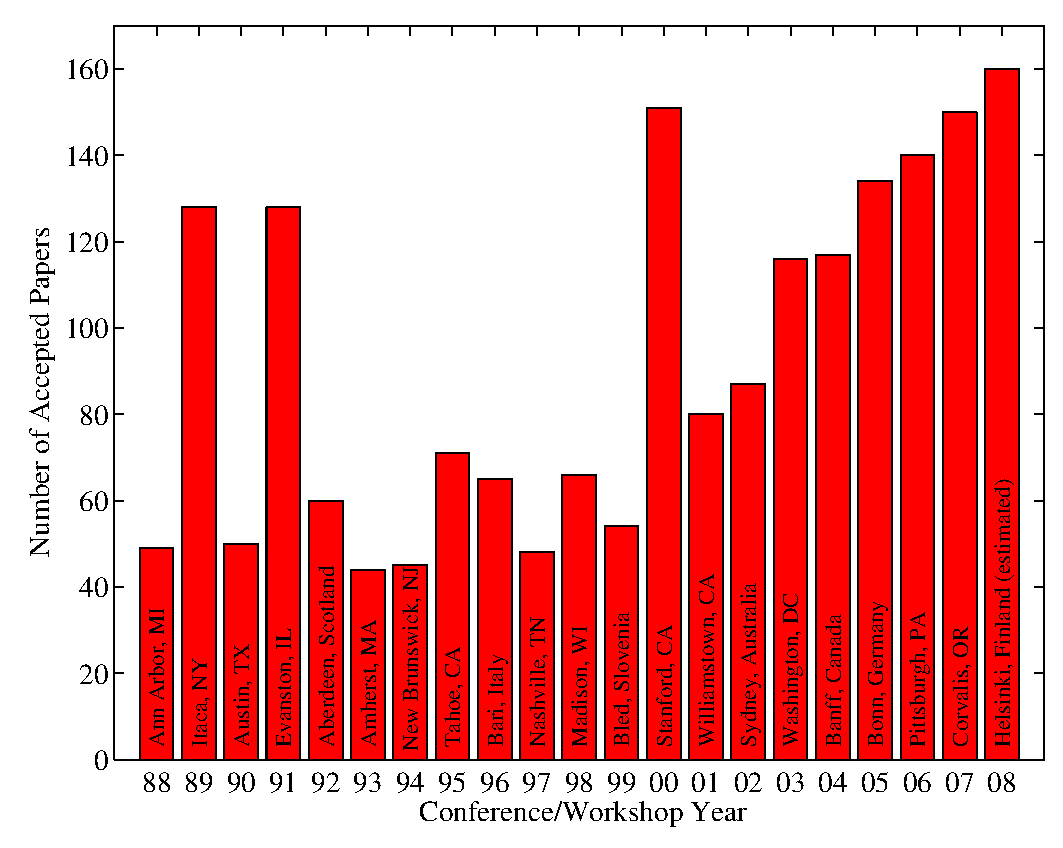
\includegraphics[width=\columnwidth]{icml_numpapers}}
% \caption{Historical locations and number of accepted papers for International
% Machine Learning Conferences (ICML 1993 -- ICML 2008) and International
% Workshops on Machine Learning (ML 1988 -- ML 1992). At the time this figure was
% produced, the number of accepted papers for ICML 2008 was unknown and instead
% estimated.}
% \label{icml-historical}
% \end{center}
% \vskip -0.2in
% \end{figure}


% If you are using \LaTeX, please use the ``algorithm'' and ``algorithmic''
% environments to format pseudocode. These require
% the corresponding stylefiles, algorithm.sty and
% algorithmic.sty, which are supplied with this package.
% Algorithm~\ref{alg:example} shows an example.

% \begin{algorithm}[tb]
%   \caption{Bubble Sort}
%   \label{alg:example}
% \begin{algorithmic}
%   \STATE {\bfseries Input:} data $x_i$, size $m$
%   \REPEAT
%   \STATE Initialize $noChange = true$.
%   \FOR{$i=1$ {\bfseries to} $m-1$}
%   \IF{$x_i > x_{i+1}$}
%   \STATE Swap $x_i$ and $x_{i+1}$
%   \STATE $noChange = false$
%   \ENDIF
%   \ENDFOR
%   \UNTIL{$noChange$ is $true$}
% \end{algorithmic}
% \end{algorithm}

% You may also want to include tables that summarize material. Like
% figures, these should be centered, legible, and numbered consecutively.
% However, place the title \emph{above} the table with at least
% 0.1~inches of space before the title and the same after it, as in
% Table~\ref{sample-table}. The table title should be set in 9~point
% type and centered unless it runs two or more lines, in which case it
% should be flush left.

% Note use of \abovespace and \belowspace to get reasonable spacing
% above and below tabular lines.

% \begin{table}[t]
% \caption{Classification accuracies for naive Bayes and flexible
% Bayes on various data sets.}
% \label{sample-table}
% \vskip 0.15in
% \begin{center}
% \begin{small}
% \begin{sc}
% \begin{tabular}{lcccr}
% \toprule
% Data set & Naive & Flexible & Better? \\
% \midrule
% Breast    & 95.9$\pm$ 0.2& 96.7$\pm$ 0.2& $\surd$ \\
% Cleveland & 83.3$\pm$ 0.6& 80.0$\pm$ 0.6& $\times$\\
% Glass2    & 61.9$\pm$ 1.4& 83.8$\pm$ 0.7& $\surd$ \\
% Credit    & 74.8$\pm$ 0.5& 78.3$\pm$ 0.6&         \\
% Horse     & 73.3$\pm$ 0.9& 69.7$\pm$ 1.0& $\times$\\
% Meta      & 67.1$\pm$ 0.6& 76.5$\pm$ 0.5& $\surd$ \\
% Pima      & 75.1$\pm$ 0.6& 73.9$\pm$ 0.5&         \\
% Vehicle   & 44.9$\pm$ 0.6& 61.5$\pm$ 0.4& $\surd$ \\
% \bottomrule
% \end{tabular}
% \end{sc}
% \end{small}
% \end{center}
% \vskip -0.1in
% \end{table}


% In the unusual situation where you want a paper to appear in the
% references without citing it in the main text, use \nocite
% \nocite{*}

\bibliography{paper_bibliography}
\bibliographystyle{icml2021}


\end{document}


% This document was modified from the file originally made available by
% Pat Langley and Andrea Danyluk for ICML-2K. This version was created
% by Iain Murray in 2018, and modified by Alexandre Bouchard in
% 2019 and 2021. Previous contributors include Dan Roy, Lise Getoor and Tobias
% Scheffer, which was slightly modified from the 2010 version by
% Thorsten Joachims & Johannes Fuernkranz, slightly modified from the
% 2009 version by Kiri Wagstaff and Sam Roweis's 2008 version, which is
% slightly modified from Prasad Tadepalli's 2007 version which is a
% lightly changed version of the previous year's version by Andrew
% Moore, which was in turn edited from those of Kristian Kersting and
% Codrina Lauth. Alex Smola contributed to the algorithmic style files.
